% Created 2022-05-10 Út 23:16
% Intended LaTeX compiler: pdflatex
\documentclass[11pt]{article}
\usepackage[utf8]{inputenc}
\usepackage[T1]{fontenc}
\usepackage{graphicx}
\usepackage{longtable}
\usepackage{wrapfig}
\usepackage{rotating}
\usepackage[normalem]{ulem}
\usepackage{amsmath}
\usepackage{amssymb}
\usepackage{capt-of}
\usepackage{hyperref}
\author{Andrej Zaujec}
\date{\today}
\title{TOI Project 2.}
\hypersetup{
 pdfauthor={Andrej Zaujec},
 pdftitle={TOI Project 2.},
 pdfkeywords={},
 pdfsubject={},
 pdfcreator={Emacs 28.0.50 (Org mode 9.6)}, 
 pdflang={English}}
\begin{document}

\maketitle
\tableofcontents


\section{Introduction}
\label{sec:org7f380fe}

The aim of this project was to try out the basics on the time-series data prediction.
The provided data were from the mobile phone accelerometer placed on the Golden Gate bridge. The data consists of four features. X, y, z coordinates and the intensity of vibration.

Firstly, I loaded the data which were then ressampled within 0.2 seconds bins and mean was used as the aggregation functions accross the bins. The data were rescaled by the Standard scaler from the scikit library.
Data points after preparation are on \hyperref[fig-data]{Figure}.

Solution of this project is included as colab notebook inside zip or can be found on this \href{https://colab.research.google.com/drive/1QnNlVVQAvBnOAw6MyzjF8tp6aVFfo1Ue?usp=sharing}{colab link}.
\begin{figure}[htbp]
\centering
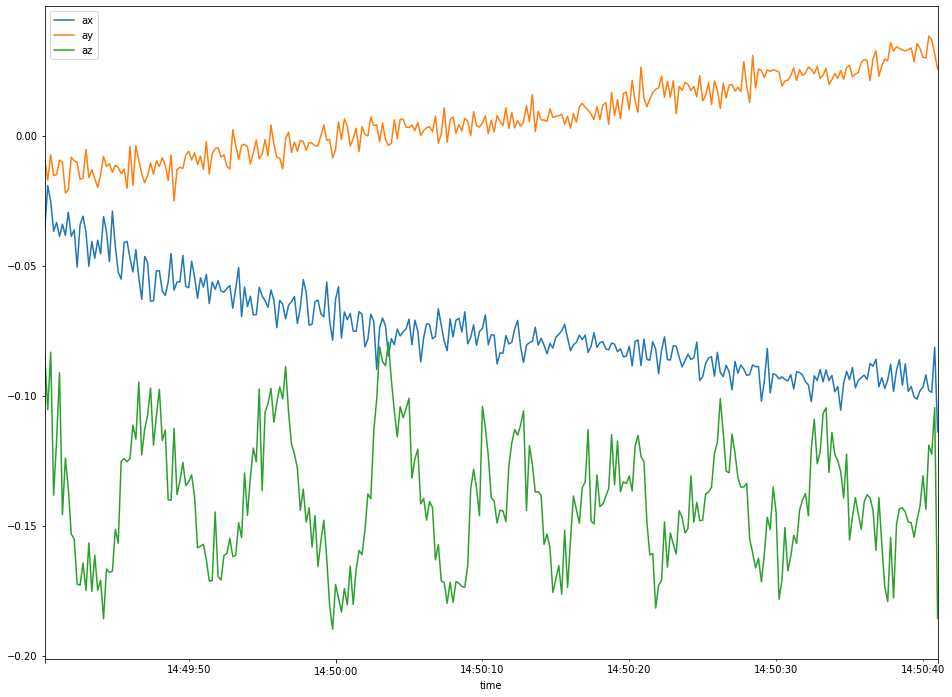
\includegraphics[width=300px]{values_plot.png}
\caption{\label{fig-data}Prepared data}
\end{figure}

\section{Models}
\label{sec:orgcea4834}
\subsection{LSTM}
\label{sec:org4ad9d84}
I choosed two LSTM layers with 100 units and one fully-connected layer as the LSTM model architecture. This model architecture was mainly inspired by the example on the 3. exercise, but I replaced 150 units with 100 as 100 proved to work better in this smaller dataset and did not to overfit as 150 units.

I tested out several variation of mentioned architecture as for example only LSTM layer or LSTM layer with linear layer. But the first mentioned architecture did work out the best in terms of results and training time.

The prediction of training data of first model, which used 20 steps window is on \hyperref[fig-first_train_model]{Figure}.
\begin{figure}[h]
\centering
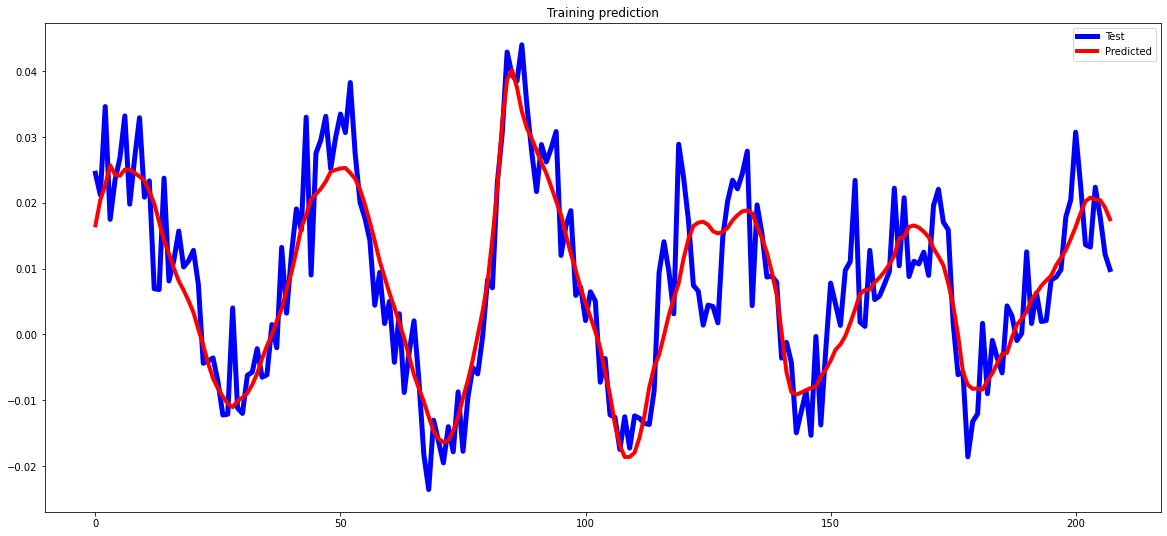
\includegraphics[width=300px]{training.png}
\caption{\label{fig-first_train_model}Prediction on training data of first model}
\end{figure}


The prediction of test data of first model, which used 20 steps window is on \hyperref[fig-first_model]{Figure}.
\begin{figure}[h]
\centering
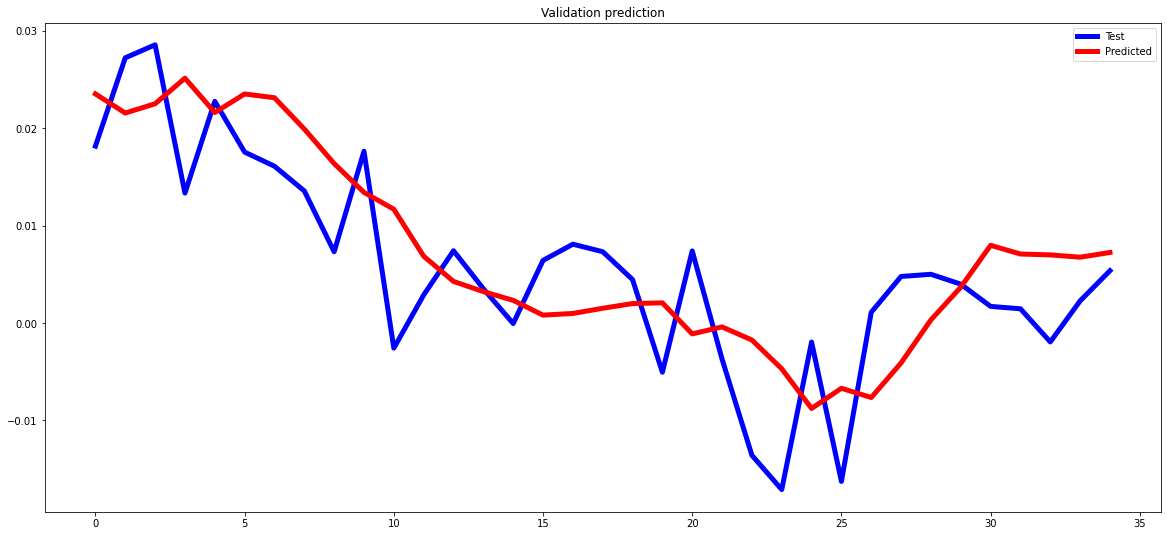
\includegraphics[width=300px]{20steps_1feat_val.png}
\caption{\label{fig-first_model}Prediction on test data of first model}
\end{figure}

Test or training predictions of models with 30 step window or 3 features are looks pretty similar and can be seen in the colab notebook nicely.

The different models evalution can be seen on \hyperref[my-table]{Table}. The compared metric is the Root Mean Squeare Error (RMSE) on the test data. The best RSME result has the first model with 20 step window and 1 feature, which is followed by model with 30 step window and 1 feature and on last place in LSTM is the model with 3 features and 20 step windows.

The 3 features seemed to confuse the model more than bring some deeper insight into it. This can be seen during different training epochs and validation loss displayed on \hyperref[fig-training]{Figure}.
The space for improvment on the LSTM models could be choosing the model with best performance in validation phase after each epoch and not the model from last epoch.
\begin{figure}[h]
\centering
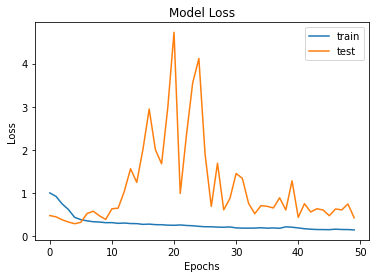
\includegraphics[width=300px]{model_loss_3feats.png}
\caption{\label{fig-training}Training process of 3 features model}
\end{figure}
\subsection{Holt-Winters Exponential Smoothing}
\label{sec:org77e2324}
This model is only stastical model in this project compared to the neural networks. I choosed additive trend, seasonality and one period contains 46 data points based on the lowest RMSE testing.
The 90\% confidance interval with forecast on test data can be seen on \hyperref[fig-holt]{Figure}.

As mentioned, more figures of each model is included in the colab notebook.
\begin{figure}[h]
\centering
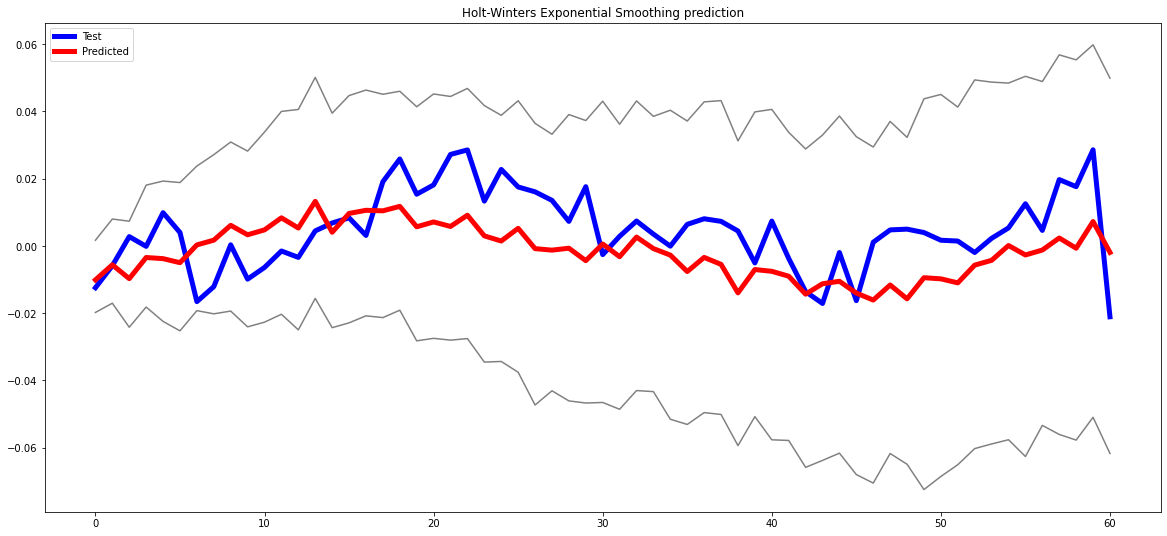
\includegraphics[width=300px]{holt_val.png}
\caption{\label{fig-holt}Prediction on test data of Holt-Winters}
\end{figure}

\begin{table}[h]
\caption{\label{my-table}Model comparisons}
\centering
\begin{tabular}{|c|c|c|}
Model & RMSE\\
\hline
1 feature, 20 steps & 0.49\\
1 feature, 30 steps & 0.52\\
3 features, 20 steps & 0.77\\
Holt-Winters ES & 0.85\\
\end{tabular}
\end{table}
\end{document}
